\fancyhead[LO, RE]{Méthodes d'alignement partiel des textes}

Nous arrivons ici à l'accomplissement de notre objectif. Avant de spécifier quel type d'alignement\index{Alignement} nous effectuerons, nous expliquerons en quoi consiste cette méthode et les moyens utilisés pour la réaliser. Ensuite, nous présenterons le logiciel avec lequel nous extrairons les informations nécessaires, pour les insérer subséquemment dans des tableaux et enfin, explorer ces données pour en tirer des conclusions.

\section{L'alignement\index{Alignement}~: travail sur l'évolution interne d'un texte}
Pour comparer les éditions et les traductions de notre corpus, nous allons utiliser une méthode~: l'alignement\index{Alignement}. Il est donc nécessaire, avant de passer à la mise en pratique, d'évoquer l'origine de cette méthode et la manière dont elle fonctionne.

\subsection{Un concept à la croisée de deux domaines}
L'alignement\index{Alignement} est un concept qui a été développé pour répondre à une problématique posée par la critique génétique textuelle et la méthode mise en place pour l'effectuer s'inscrit dans le domaine du \acrfull{tal}.

La critique génétique textuelle ou génétique des textes est une discipline littéraire qui est née il y a de nombreuses années, afin d'amener une nouvelle méthode de lecture des textes et notamment des manuscrits. L'objectif est d'analyser l'écriture du texte et sa production et cela suit plusieurs étapes. La première s'étend de la conception de l'œuvre par l'auteur jusqu'à la publication. L'étape suivante prend en compte \og~les interventions de l'auteur sur des éditions successives~: depuis l'édition première dite \textit{princeps}, jusqu'à une édition de référence, dite définitive\footcite[p.~1]{genetique_texte}~\fg{}. Enfin, l'analyse porte sur \og~les variations successives du texte dues soit à des erreurs soit à des initiatives des copistes successifs.\footcite[p.~1]{genetique_texte}~\fg{}. Par cette discipline, il y a une recherche sur un corpus de plusieurs versions d'un texte et \og~les généticiens du texte cherchent à reconstituer la genèse de l'œuvre sous ses différents aspects.\footcite{alignement_bourdaillet}~\fg{}. Afin d'effectuer ces recherches, il est donc essentiel de trouver diverses manières d'analyser le texte pour faire ressortir les éléments voulus et c'est ce à quoi sera utilisé l'alignement\index{Alignement}, qui consiste à rechercher les invariants et les différences entre deux textes.

L'étude de plusieurs textes pour repérer des similitudes ou des différences est un travail ardu et assez précis~; l'effectuer manuellement prendrait un temps considérable et serait très fastidieux. Des moyens de répondre à l'alignement\index{Alignement} informatiquement ont donc été recherchés et c'est ainsi que le concept se lie au \acrshort{tal}. Le \acrshort{tal} est une discipline qui associe linguistes et informaticiens et qui a comme objectif l'automatisation des processus, c'est-à-dire \og~mettre en place une chaîne de traitement permettant, à partir d'un ensemble de données injectées en entrée, d'obtenir un résultat distant en sortie.\footcite[p.~1022]{tal_etude_comparee}~\fg{}. L'intérêt est donc de créer des outils, des logiciels ou des programmes informatiques pour travailler automatiquement sur des données linguistiques. Différents algorithmes ont alors été écrits pour obtenir divers résultats, plus ou moins détaillés, de cet alignement\index{Alignement}, afin de faciliter le travail des linguistes en fonction des sources soumises et du corpus à disposition.

\subsection{Fonctionnement de l'alignement\index{Alignement}~: trouver des méthodes efficaces}
Il est nécessaire de prendre en compte un certain nombre d'éléments pour réaliser correctement l'alignement\index{Alignement} et pour savoir quelles données sont significatives pour le travail fait. 

\subsubsection{Quels types de corpus pour l'alignement\index{Alignement} ?}
Un des aspects importants est le corpus et il est possible de réaliser un alignement\index{Alignement} sur quatre types de corpus. Il y a tout d'abord le corpus monolingue ou unilingue\index{Alignement!corpus monolingue} et le corpus multilingue\index{Alignement!corpus multilingue}, dont dans le deuxième cas, la langue est un élément qui rendra l'alignement\index{Alignement} encore plus ardu. 
Ensuite, pour les cas de corpus multilingue\index{Alignement!corpus multilingue}, il y a soit des corpus parallèles, soit des corpus comparables. Dans le premier cas, les textes seront des traductions mutuelles alors que dans le second, les textes ne sont pas les mêmes mais ils possèdent un vocabulaire identique entre les langues. Au milieu de ces deux corpus, il existe un type de corpus quelque peu intermédiaire~: les corpus parallèles bruités, c'est-à-dire des corpus parallèles mais qui ne respectent pas complètement ses contraintes, par des manques ou des décalages dans les documents\footcite[p.~4-6]{alignement_prochasson}. Notre travail d'alignement\index{Alignement} avec le projet MetaLEX\index{Projet MetaLEX} porte à la fois sur des corpus monolingues\index{Alignement!corpus monolingue} puisqu'il existe plusieurs éditions dans une même langue, mais également sur un corpus multilingue\index{Alignement!corpus multilingue} puisqu'une fois tous ces corpus monolingues\index{Alignement!corpus monolingue} réunis, nous les étudierons tous ensemble. Ces corpus sont principalement des corpus parallèles, puisqu'ils sont fondamentalement les mêmes vis-à-vis du texte~: ici donc, c'est la traduction qui nous intéressera notamment. Cependant, il y a aussi des cas de corpus parallèles bruités, puisque nous avons des modifications de certains éditeurs, ce qui signifie que certains textes ne suivent pas les contraintes du corpus parallèle. Ainsi, nous avons une certaine diversité dans notre corpus, ce qui signifie qu'il faudra correctement choisir notre méthode d'alignement\index{Alignement} pour obtenir des résultats satisfaisants. 

\subsubsection{Quelles bases de comparaisons pour l'alignement\index{Alignement} ?}
L'objectif d'un alignement\index{Alignement} est d'observer deux textes et de les comparer dans leur structure et leur fond. Il est donc essentiel de déterminer ce qui sera recherché pour mettre au point cet alignement\index{Alignement}. 

Il existe trois types de différences entre deux textes~: suppressions, insertions et remplacements. La suppression signifie la disparition d'un mot, d'un morceau, d'une phrase ou d'un bloc au sein d'un texte. L'insertion signifie le rajout d'un de ces éléments. Le remplacement se caractérise par une suppression suivie d'une insertion. Avec l'alignement\index{Alignement} que nous avons choisi, il y a également le cas du déplacement qui est à prendre en compte, c'est-à-dire qu'il y a eu une suppression d'un bloc de texte et une insertion ensuite de ce bloc à une autre position. Dans cet alignement\index{Alignement}, il y aura enfin le cas des invariants, c'est-à-dire que certains blocs de texte n'auront absolument pas été modifiés. Ce type d'alignement\index{Alignement} est pratique puisqu'il prend en compte tous les éléments de changements qu'il peut y avoir eu dans un texte et permet donc d'effectuer une analyse exhaustive. L'algorithme de cet alignement\index{Alignement}, comme nous le retrouvons avec \textsc{medite}, fonctionne de manière à aller traiter le texte, identifier les blocs répétés, identifier les invariants et les déplacements~; puis, une fois que tous ces blocs ont été trouvés, il déduira les blocs non répétés, pour nous fournir toutes les données dont nous avons besoin\footcite{alignement_monolingues_bourdaillet_ganascia}. Cependant, cet alignement\index{Alignement} aura un inconvénient~: il est monolingue\index{Alignement!corpus monolingue}. Il ne sera pas possible d'utiliser cet algorithme pour un corpus multilingue\index{Alignement!corpus multilingue}, puisqu'il considérera qu'il n'y a aucun invariant à moins qu'un mot soit le même entre les deux langues. Il faudra donc trouver un moyen d'effectuer les comparaisons entre des corpus de langues différentes.

Ainsi, parmi les méthodes utilisées pour l'alignement multilingue\index{Alignement!alignement multilingue}, il existe celles des points d'ancrage. Cela revient à trouver des informations entre les corpus qu'il est possible de relier de manière fiable pour réaliser l'alignement\index{Alignement}, puisque les langues entre les textes ne seront pas les mêmes. Il est possible de s'appuyer sur des informations structurelles, telles qu'un titre ou une légende mais aussi sur un lexique, en se basant sur un vocabulaire bilingue\footcite[p.~9-10]{alignement_prochasson}. Par cette méthode, la recherche sera facilitée et il sera plus aisé de se baser sur des éléments familiers pour aligner les textes.

\paragraph{}Depuis l'apparition de l'alignement\index{Alignement} comme méthode de critique génétique des textes, il y a donc eu une quantité d'algorithmes produits et de méthodes développées pour étudier un texte, en fonction des besoins et des éléments à disposition. Nous ne les avons pas tous évoqués mais nous nous sommes plutôt concentrés sur ceux que nous allons utiliser dans notre démonstration, afin de réaliser l'objectif de notre projet. L'intérêt sera d'aligner à la fois les corpus monolingues\index{Alignement!corpus monolingue} et les corpus multilingues\index{Alignement!corpus multilingue} mais surtout de travailler avec une procédure qui sera semi-automatique, afin de toujours répondre à la problématique du \acrshort{tal}.

\section{Sonder notre corpus~: réflexions sur la forme de l’alignement\index{Alignement}}
\subsection{Alignement par unité de texte~: un corpus inadapté}
Avant de pouvoir réaliser un quelconque alignement\index{Alignement}, il est nécessaire de délimiter les règles que nous allons suivre pour créer cet alignement\index{Alignement}. Il est capital tout d’abord de sélectionner l’unité de base avec laquelle nous ferons notre analyse. Un alignement\index{Alignement} basique se ferait selon la phrase ou le paragraphe pour un récit ou la ligne dans le cas, par exemple, d’un poème. Cela fut une des propositions avancées pour notre alignement\index{Alignement}, de rechercher les différences de phrases entre nos diverses éditions. Cela posait cependant deux problèmes. Tout d’abord, pour les cas où il y avait eu une restructuration du texte, la phrase aurait essentiellement été modifiée et l’alignement\index{Alignement} deviendrait alors plus compliqué puisqu’il ne serait pas aisé de trouver les limites de la phrase, surtout si elles ont disparu. Ensuite, l’aspect multilingue est problématique vis-à-vis de cet alignement\index{Alignement}. Il peut être difficile de trouver les équivalents de la phrase entre les versions, les différences de ponctuations peuvent influer et en substance, aligner toute une phrase d’une langue à l’autre serait un travail complètement manuel, alors que nous recherchons une méthode semi-automatique pour réaliser cet alignement\index{Alignement}. Cela avait été prouvé par \textsc{medite} qui n’a absolument pas la capacité dans son algorithme de travailler sur deux textes s’ils n’ont pas la même langue. Il ne sera donc pas possible de choisir une unité de texte comme seule base de l’alignement\index{Alignement}.

\subsection{Alignement partiel\index{Alignement!alignement partiel} ciblé\index{Alignement!alignement cible@alignement ciblé}~: une solution d’harmonie avec le projet principal}
La réflexion a donc porté ensuite sur l’idée d’un alignement partiel\index{Alignement!alignement partiel}, qui ne prend en compte qu’un certain type d’éléments pour observer les différences entre les éditions. La détermination de ces éléments s’est rapidement faite, puisque nous avons réfléchi à l’objectif du projet MetaLEX\index{Projet MetaLEX} qui est d’étudier l’évolution des langues historiques du droit en Europe et nous avons donc choisi de réaliser un alignement partiel\index{Alignement!alignement partiel} ciblé\index{Alignement!alignement cible@alignement ciblé} à partir d’un lexique juridique. Le lexique juridique a été établi par les linguistes du projet en suivant le chapitre que nous analysons en priorité et si cette technique d’alignement\index{Alignement} fonctionne, la suite consistera à élargir cette liste afin d’avoir un lexique juridique déterminé avec lequel nous réaliserons la démarche sur l’ensemble de l’ouvrage. Nous avons pu examiner ce lexique juridique dans le chapitre \ref{chap_annotations}, lorsque nous avons mis en place les annotations. Ces dernières seront essentielles à notre travail puisque c’est grâce à elles que nous aurons la possibilité de faire notre alignement\index{Alignement} semi automatiquement mais aussi suivant un corpus multilingue\index{Alignement!corpus multilingue}, où elles représenteront nos points d’ancrage. En travaillant l’alignement\index{Alignement} suivant un lexique, il suffit simplement de trouver les traductions littérales des termes entre les langues et ensuite le travail se fait plus aisément à travers l’identifiant que nous avons apposé plus tôt. Le principe donc de notre alignement\index{Alignement} sera de rechercher les termes juridiques dans les textes à partir d’un identifiant, de trouver les contextes identiques de présence du mot et d’inscrire ces informations dans un tableau de données.

Ce choix du lexique par les identifiants présente tout de même une limite puisque pour sélectionner l’annotation, nous avons réduit le mot à son lemme et cela vaut pour toutes les catégories grammaticales. Ainsi, lorsque l’on relèvera le terme dans notre alignement\index{Alignement}, nous ne prendrons pas en compte les différences au sein même du terme, c’est-à-dire par exemple que nous ne mentionnerons pas le cas où la forme désuète du mot s’est modernisée dans une version plus récente, comme nous l’aurons notamment avec le terme \textit{loi} en français. Cela représente un choix que nous avons fait avec l’alignement\index{Alignement} actuellement réalisé mais cela pourra être rectifié par la suite, lors de l’amélioration du tableau d’alignement\index{Alignement!tableau d'alignement}.

\paragraph{} Ainsi donc, nous avons décidé de ne pas suivre les exemples standards d’alignement\index{Alignement} que nous avons pu présenter dans la première section et nous n’aurons donc pas recours à un des algorithmes qui permettent d’effectuer ces calculs de différences entre plusieurs éditions. Pour réaliser notre alignement\index{Alignement}, nous allons nous appuyer sur le lexique juridique précédemment établi, sur la structure des phrases par le biais d’une numérotation et sur une des fonctionnalités proposées par \textsc{txm}.

\section{Étudier le contexte textuel du lexique juridique~: extraction de données à partir d’un concordancier\index{Concordancier}}
Parmi les outils de statistiques textuelles\index{Statistique textuelle} que nous avons mentionnés et utilisés précédemment, nous avons brièvement évoqué le concordancier\index{Concordancier}. Cet outil permet, pour un mot choisi, de connaître son contexte dans le texte, c’est-à-dire de découvrir les morceaux de phrases qui l’entourent. Cela est fourni dans la majorité des logiciels de textométrie\index{Textometrie@Textométrie} et de lexicométrie et notamment dans les deux auxquels nous avons eu recours. \textsc{rstudio} donne la possibilité, par des lignes de script, de demander les concordances pour un mot donné et il fournit ensuite dans la console les extraits de texte où se trouve ce mot. La méthode fournie par \textsc{txm} est beaucoup plus élaborée et apporte des précisions qui seront primordiales pour notre travail.

\subsection{Le concordancier\index{Concordancier} de TXM~: un outil adapté pour l’alignement\index{Alignement}}
L’interface graphique de \textsc{txm} permet de présenter les résultats du concordancier\index{Concordancier} d’une manière beaucoup plus précise que ne le faisait \textsc{rstudio} et cela nous permet également de mener à bien notre objectif. Elle offre un certain nombre de paramètres qui permettent une précision dans la recherche et avec les résultats, nous observons le pivot, c’est-à-dire le mot que nous avons recherché, son contexte gauche et son contexte droit, ainsi que sa référence. Il est possible également de classer selon ces paramètres, si le choix est plutôt d’étudier par texte ou de voir préférablement le résultat d’un côté de la phrase ou de l’autre, mais également de les modifier selon notre volonté, comme cela est illustré avec la figure \ref{fig:concordancier_parametres}. \textsc{txm} offre ainsi la possibilité de modifier leur forme d’apparition~: les contextes et le pivot sont présentés sous leur forme classique, celle du mot, mais il serait également possible d’avoir le lemme, la catégorie lexicale ou même le \emph{mlx}, que nous avons inséré, pour le pivot, ce qui ne nous montrerait plus les différentes orthographes du mot. De plus, nous pouvons choisir la quantité d’éléments que nous voulons voir apparaître dans ces contextes, pour les cas par exemple où il faut plus de données dans la phrase pour réellement en comprendre le sens. L’un des champs modifiables les plus intéressants dans le cas de notre recherche sera celui des \textbf{Références}. Ce dernier ressort toutes les identifications que fournit \textsc{txm} lorsqu’il encode les textes que nous lui fournissons et il donnera donc la possibilité de faire apparaître les différentes formes du pivot, de mettre la date ou la langue du texte mais il peut aussi fournir des éléments beaucoup plus importants tels que les identifiants du texte ou les numéros de phrases. \textbf{Références} donne enfin la possibilité avec ces paramètres de choisir l’ordre d’apparition dans le tableau des résultats et de choisir les clés et l’ordre de tri. Ainsi, il sera possible de faire apparaître la phrase selon un ordre alphabétique des mots de chacun des contextes ou il sera possible de sélectionner comme référence le numéro de phrase et l’identifiant de textes et c’est ce que nous allons privilégier dans notre travail, en les classant dans cet ordre pour faciliter notre alignement\index{Alignement}.
\begin{figure}[H]
    \centering
    \caption{Paramètres de commande pour une requête de concordance sur \textsc{txm}}
    \fbox{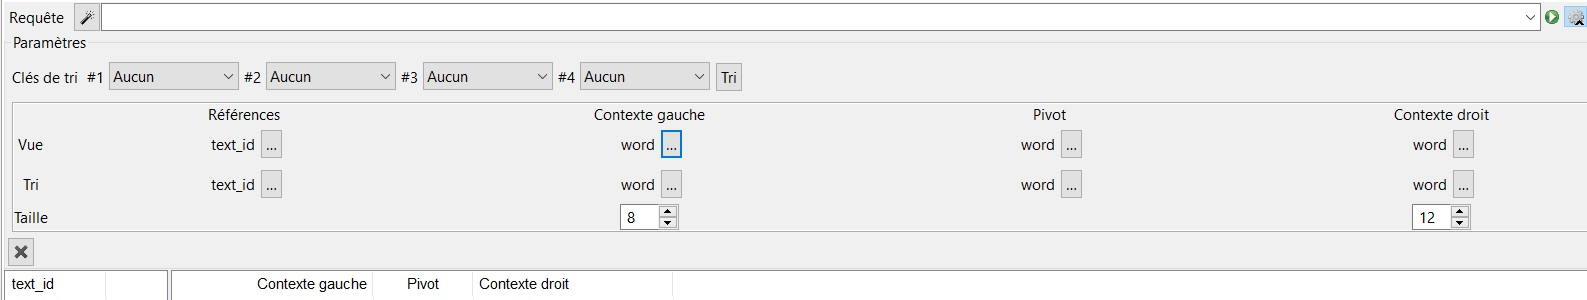
\includegraphics[width=16cm, height=3.5cm]{Partie3/images/chap4/concordancier_parametres.jpg}}
    \label{fig:concordancier_parametres}
\end{figure}

\subsection{Exemple d’une requête tirée du lexique}
Afin d’illustrer l’intérêt du concordancier\index{Concordancier} pour la réalisation de notre alignement\index{Alignement}, le meilleur moyen est de fournir un exemple à partir du corpus multilingue\index{Alignement!corpus multilingue} qui a été annoté avec les termes du lexique juridique et qui a ensuite été importé sur le logiciel sous le nom de CORPUSALPHA. Nous choisissons pour l’exemple un terme monolexical pour les trois langues~: \og~T\_adultery~\fg{}. Nous avons choisi comme clé de tri le numéro de phrase et l’identifiant de texte et nous avons effectué un classement dans l’ordre croissant pour l’un puis chronologique pour l’autre. 
\begin{figure}[p]
    \centering
    \fbox{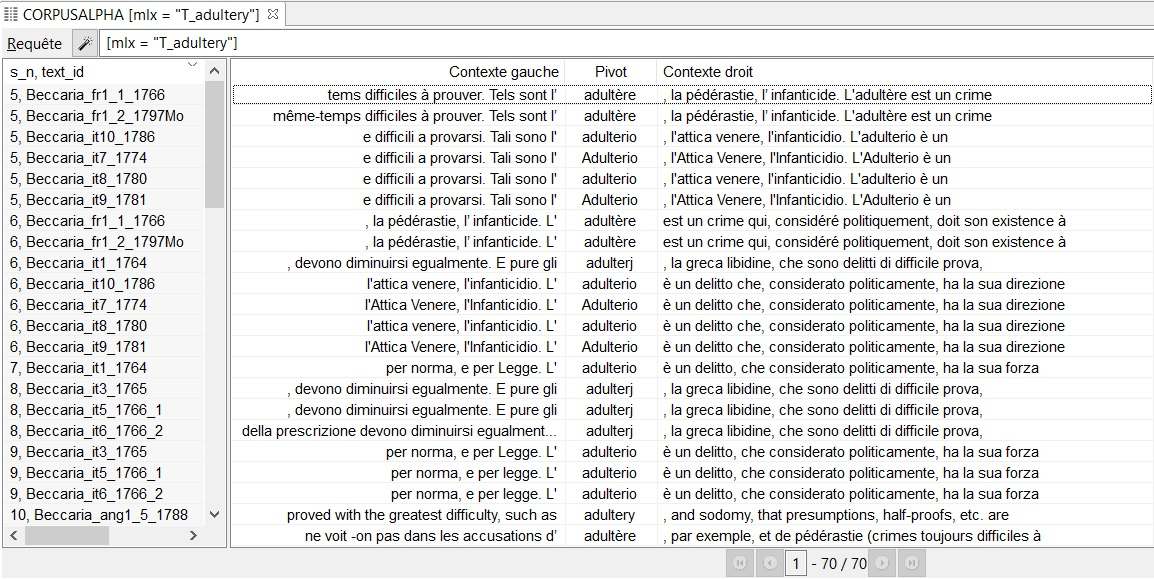
\includegraphics[width=17cm, height=10cm]{Partie3/images/chap4/concordancier_adultery.jpg}}
    \caption{Recherche de concordances pour l’identifiant \og~T\_adultery~\fg{} à travers le corpus multilingue CORPUSALPHA}
    \label{fig:concordancier_adultery}
\end{figure}
Nous pouvons donc observer avec cette requête, illustrée avec la figure \ref{fig:concordancier_adultery}, plusieurs éléments. Tout d’abord, nous pouvons voir que la forme \textit{adultère} a été annotée 70 fois avec l’identifiant. Le mot apparaît également ici dans toutes les langues donc il n’y a pas eu d’erreur d’annotation pour l'une d'elles, comme nous en avons eu à quelques reprises qui ont pu fausser l’alignement\index{Alignement}. Nous pouvons également observer qu’avec l’identifiant, les différences de formes ou de présentation du mot ne comptent pas, comme la majuscule par exemple. Ensuite, nous pouvons constater, dans la colonne des \textbf{Références}, que le classement par numéro de phrase a effectué un mélange de langues entre les éditions, ce qui peut illustrer le fait que même les différences de langues n’ont pas influé sur la structure de la phrase pour certaines éditions. Enfin, avec ce classement, on peut déjà reconnaître quelle phrase sera alignée avec une autre grâce au contexte, puisque l’on retrouve des phrases d’une même langue qui sont identiques, mais également entre deux langues. Il est déjà possible d’affirmer, par exemple, juste en observant la figure que certaines phrases en français et en italien seront sur la même ligne du tableau\index{Alignement!tableau d'alignement}, en observant simplement leur contexte droit~:
\begin{itemize}
    \item \og~adultère [\dots] considéré politiquement~\fg{} (fr)
    \item \og~adulterio [\dots] considerato politicamente~\fg{} (it)
\end{itemize}
En suivant ces traductions plus ou moins littérales, nous aurons ainsi la possibilité d’établir notre alignement\index{Alignement} de la manière la plus complète possible, puisque le concordancier\index{Concordancier} permet en plus de pallier certains obstacles que nous avons évoqués précédemment.

\subsection{\label{section_resolution}Une résolution partielle de certaines limites de l’alignement\index{Alignement}}
Les différentes options d’affichage du concordancier\index{Concordancier} donnent la possibilité de pousser notre travail un peu plus loin qu’en faisant simplement apparaître les expressions monolexicales puisqu’elles vont nous permettre de ne pas limiter l’alignement\index{Alignement} à ces expressions. Le concordancier\index{Concordancier} nous offre également l’opportunité de corriger les cas où certains mots n’ont pas été annotés car ils n’étaient pas reconnaissables par le script Python dans le dictionnaire qui avait été soumis. Ces deux solutions s’articuleront dans certains cas afin de parfaire notre alignement\index{Alignement}.

Dans le chapitre \ref{chap_annotations}, nous avions présenté un obstacle inhérent à la liste de termes juridiques et au balisage du texte que nous annotions~: lorsque certains termes sont polylexicaux, il n’est pas possible d’annoter comme nous avions pu le faire pour les expressions monolexicales. Nous avions alors proposé une solution un peu limitée, qui consistait à annoter un seul mot de l’expression, proposition que nous avions ensuite rejetée car cela serait trop compliqué de retrouver le reste de l’expression. Cette limite disparaît à partir du moment où nous travaillons avec le concordancier\index{Concordancier}. Comme nous l’avons expliqué, le concordancier\index{Concordancier} de \textsc{txm} permet de faire apparaître les contextes droit et gauche de la phrase dont est tirée la forme annotée. Ainsi, à partir du moment où nous avons connaissance de l’expression exacte que nous recherchons, il est possible, lors de l’apparition des résultats du mot annoté, de distinguer les phrases et expressions qui correspondent à ce que nous avons dans notre lexique juridique et ainsi de rajouter les expressions polylexicales dans notre alignement\index{Alignement}.
\begin{figure}[p]
    \centering
    \fbox{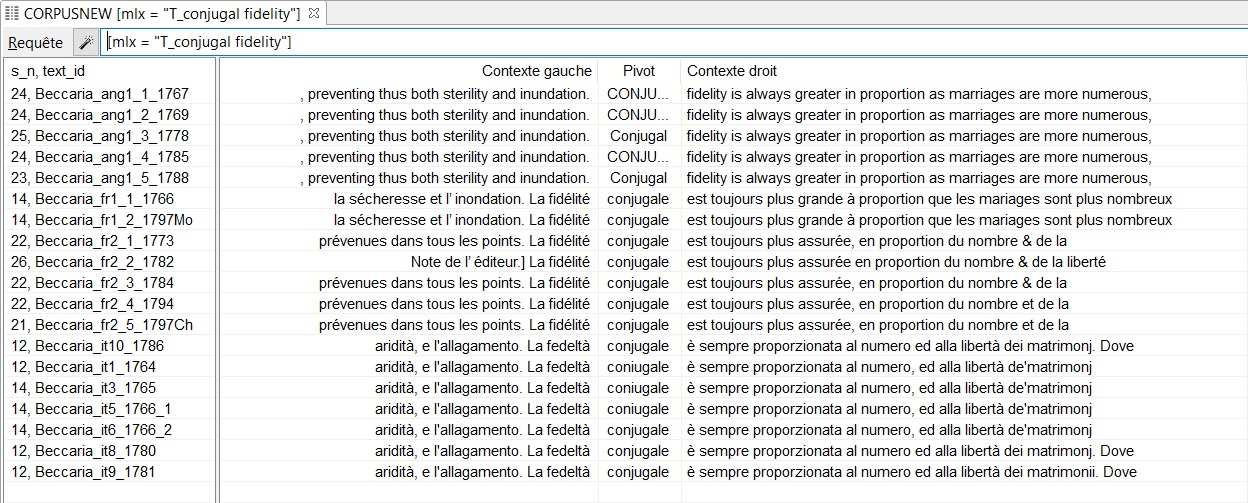
\includegraphics[width=17cm, height=10cm]{Partie3/images/chap4/concordancier_conjugal_fidelity.jpg}}
    \caption{Recherche de concordances pour l’identifiant \og~T\_conjugal fidelity~\fg{} à travers le corpus multilingue\index{Alignement!corpus multilingue} CORPUSALPHA}
    \label{fig:concordancier_conjugal_fidelity}
\end{figure}

L’exemple que nous avons avec la figure \ref{fig:concordancier_conjugal_fidelity} est celui de l’expression de \textit{fidélité conjugale}, significative dans le cas de ce chapitre spécifique et en deux mots, ce qui oblige à un choix d’annotation. J’ai choisi ici d’annoter le terme \textit{conjugal} plutôt que \textit{fidélité} puisque j’ai considéré qu’il était possible que le terme de fidélité se retrouve autrement dans le texte, si nous prenons en compte le fait que le chapitre débat de l’adultère, alors qu’il était plus probable que l’adjectif \textit{conjugal} ne se retrouve que lié à la fidélité. L’intérêt particulier de cette annotation est l’identifiant que nous lui avons donné. J’ai annoté la forme \textit{conjugal} avec l’expression complète de \textit{fidélité conjugale}. Cela signifie que, dans le cas où la forme se trouve sous un autre contexte dans le texte, il faudra chercher le terme \textit{fidélité} dans les contextes qui l’entourent pour s’assurer de faire correctement l’alignement\index{Alignement} et de choisir les bons éléments. De ce fait, cette méthode accroît la source d’annotations qui nous permettra de réaliser le tableau d’alignement\index{Alignement!tableau d'alignement}. Cela n’est cependant pas complètement efficient, puisqu’il existe certaines expressions qui sont composées d’autres expressions annotées ou qui sont trop compliquées pour faciliter l’encodage et cela obligera alors à effectuer un travail un peu plus manuel pour trouver les éléments manquants.

Nous devrons alors effectuer également une recherche plus ou moins manuelle pour contourner l’autre limite. Pour réaliser l’annotation, nous avons rédigé un script informatique, que nous avons associé à un dictionnaire de termes juridiques et que nous avons appliqué au texte que nous avons ensuite importé dans le logiciel \textsc{txm}. Toute cette démarche est majoritairement automatique, tout comme la recherche d’une expression clé avec le concordancier\index{Concordancier} ensuite, ce qui nous permet d’avoir accès à un grand nombre de mots rapidement et facilement. Pour rechercher les termes qui n’ont pas été correctement annotés, nous procédons à un travail bien plus manuel puisque nous devons aller observer le contenu de l’édition pour trouver la forme du terme dans un des textes spécifiques d’une édition pour pouvoir le rechercher ensuite dans le concordancier\index{Concordancier} et trouver les informations dont nous avons besoin pour l’alignement\index{Alignement}. Par cette technique, nous pourrons ainsi aller chercher les cas où les annotations n’ont pas fonctionné. Nous pouvons citer comme exemple \textit{half-proof}/\textit{half proof} en anglais qui pose plusieurs difficultés. L’écriture n’est pas la même entre les versions, puisqu’elle prend parfois un tiret. Le terme \textit{proof} a déjà été identifié dans le texte et la forme \textit{half} est utilisée à plusieurs reprises. L’identifiant avec un seul terme n’est donc pas ici possible et cette technique manuelle sera la seule productive pour ce cas-là.

\paragraph{}Le concordancier\index{Concordancier} de \textsc{txm} offre ainsi de nombreuses fonctionnalités qui nous permettront d’extraire une grande quantité de données profitables à notre travail afin d’aller dans les détails et de fournir un tableau d’alignement\index{Alignement!tableau d'alignement}, qui sera le plus complet possible.

\section{Mettre en forme les données recueillies~: réalisation de tableaux d’alignement\index{Alignement!tableau d'alignement}}
À l’aide de toutes les informations que nous avons recueillies lors du travail sur \textsc{txm}, nous avons la possibilité d’établir un alignement\index{Alignement} sous la forme d’un tableau\index{Alignement!tableau d'alignement}, dont nous présenterons tout d’abord une version simple, puis une version avancée plus détaillée.

\subsection{Transcrire les informations extraites~: établissement du tableau d’alignement\index{Alignement!tableau d'alignement} simple}
Dans un premier temps, nous avons décidé d’établir un tableau d’alignement\index{Alignement!tableau d'alignement} simple, qui rapporte les numéros de phrases où se trouve l’expression choisie dans le texte, en fonction des éditions, et les cas où elle n’y est pas. Le tableau\index{Alignement!tableau d'alignement} porte sur le chapitre 30/31/36 et se compose de colonnes qui comprennent toutes les éditions que nous avions dans notre étude du concordancier\index{Concordancier} et de lignes qui contiennent les termes juridiques, avec plusieurs lignes pour un même terme dans les cas où ce dernier apparaît plusieurs fois dans le texte. 

L’intérêt est alors de récupérer dans le concordancier\index{Concordancier} les différentes phrases où apparaît le terme choisi, de chercher les similitudes entre deux éditions, de la même langue ou d’une langue différente. Dans les cas où il y a des utilisations identiques du terme, nous inscrivons dans le tableau d’alignement\index{Alignement!tableau d'alignement}, les numéros de phrases selon ce qui a été établi par \textsc{txm}. Sur la même ligne, se trouvera le numéro de phrase pour chacune des éditions qui utilise le terme dans le même contexte. 

Il existe cependant des cas où une édition n’apparaît pas dans les résultats du concordancier\index{Concordancier}. Nous vérifions alors que ce terme n’a pas été mal inscrit, selon la méthode manuelle évoquée dans la section précédente. Dans les cas où cela est avéré, nous cherchons son numéro de phrase, pour l’inscrire dans le tableau\index{Alignement!tableau d'alignement}. Dans les cas où il n’y a pas eu d’erreur et où le terme ne figure effectivement pas, nous inscrivons un signe pour signifier l’absence du terme (un \emph{slash} dans le cas de notre tableau\index{Alignement!tableau d'alignement}). 

Nous pouvons en observer un échantillon dans le tableau\index{Alignement!tableau d'alignement} \ref{table:alignement_simple}, avec l’exemple du terme \textit{preuve}, identifié par l’annotation \og~T\_proof~\fg{}.
Le tableau\index{Alignement!tableau d'alignement} nous permet de voir que le terme \textit{preuve} apparaît de huit manières différentes au sein de toutes les éditions et qu’il y a des cas où cette utilisation est commune à toutes les versions ou presque et d’autres cas où cela représente une spécificité d’une édition ou même d’une langue en particulier. Ainsi, par exemple, avec ce terme là, nous pouvons voir que l’édition française de 1782 emploie le terme identifié par \og~T\_proof~\fg{} d’une manière qui n’est reprise par aucun autre texte. La dernière ligne de la figure permet de constater qu’il y a également un cas où seules les éditions anglaises utilisent le terme. 

Par ailleurs, nous pouvons remarquer qu’il y a de nombreuses situations où le terme n’aura pas été utilisé, sans autre explication dans le tableau\index{Alignement!tableau d'alignement}. C’est ce détail qui sera ajouté dans le nouveau tableau\index{Alignement!tableau d'alignement} plus précis et plus développé de notre alignement\index{Alignement}.

\subsection{Consigner les modifications effectuées~: enrichissement avec le tableau d’alignement\index{Alignement!tableau d'alignement} avancé}
Dans un second temps et afin de parfaire notre travail, nous avons décidé de rajouter de nouveaux éléments dans le tableau\index{Alignement!tableau d'alignement} ayant pour objectif d’apporter les informations que nous n’avions pas dans le premier tableau\index{Alignement!tableau d'alignement}, c’est-à-dire remplacer tous les \textit{slashs} qui signalaient une non-présence du terme juridique et indiquer ce qu’il y a à la place. En observant les différentes éditions et en recherchant les zones de textes où le terme juridique aurait dû apparaître, nous avons pu distinguer différents types de changements que nous avons classé en quatre catégories~:
\begin{itemize}
    \item R = Remplacement~: le terme a été remplacé par un autre mot~;
    \item S = Suppression~: le terme a été supprimé dans cette version du texte et n’existe plus~;
    \item I = Inexistant~: le contexte du terme est inexistant dans une édition~;
    \item E = Équivalent~: le terme a changé mais la racine est la même.
\end{itemize}
En plus de ces différentes informations, nous rajoutons deux autres détails pour compléter notre tableau d’alignement\index{Alignement!tableau d'alignement}. Dans les cas d’une suppression ou d’une inexistence du terme, nous mettons simplement l’identifiant de la catégorie. Dans les cas d’un remplacement ou d’une équivalence, nous allons spécifier le numéro de phrase du nouveau terme, afin de savoir si, bien qu’il y ait un changement, la structure et le contexte de la phrase n’ont pas changé. Puis nous renseignons le terme qui structure la phrase à la place de celui que nous recherchons.

Dans le but d’observer cela, nous pouvons reprendre l’exemple que nous avions présenté dans la première sous-section, avec cette fois-ci les éléments qui composent le tableau d’alignement\index{Alignement!tableau d'alignement} avancé, ce que nous observons avec le tableau\index{Alignement!tableau d'alignement} \ref{table:alignement_avance}.
En reprenant les observations de la première sous-section, nous pouvons donc y ajouter des éléments. L’édition française de 1782 semblait avoir une utilisation unique du terme choisi et après recherche dans les différents textes, nous pouvons effectivement voir que cela est dû à une note de bas de page dans l’édition, ce qui explique que la catégorisation pour le reste de la ligne sera \og~inexistant~\fg{}. Nous pouvons observer également des cas d’équivalences, avec la septième utilisation de \og~T\_proof~\fg{} dans le texte, où cela est équivalent avec \textit{semi-preuves} ou \textit{half-proof}. Nous voyons ici le cas que nous avions évoqué dans la sous-section \ref{section_resolution}, où le tiret changeait l’encodage du mot et donc l’annotation subséquente. Ici donc, nous avons une équivalence, puisque le terme \textit{preuve} est utilisé mais avec un élément supplémentaire. Cet exemple nous permet également d’observer des cas de suppressions de l’utilisation du mot, ainsi que des remplacements, où le terme de \textit{preuve} ne convenait pas et où il y a un nouveau terme, qui est cependant à la même place que l’est \textit{preuve} dans les autres contextes. Nous pouvons distinguer, avec la troisième apparition de \og~T\_proof~\fg{} que les éditions utilisent le même terme en lieu et place de \textit{preuve}~: \textit{produce}. Cela peut indiquer une considération des traducteurs pour mieux retranscrire l’idée générale de la phrase.

\paragraph{}Ainsi donc, avec ces différents tableaux, nous discernons des cas où l’alignement\index{Alignement} n’est pas parfait puisque le terme utilisé est le même mais il n’est pas présent dans les mêmes phrases mais aussi des cas où nous avons un alignement\index{Alignement} entre les phrases mais où le terme utilisé n’est pas identique. Les tableaux produits fournissent déjà, de ce fait, un certain nombre d’informations sur les éditions, sur leurs similitudes et leurs différences mais il sera nécessaire de les étudier plus en profondeur pour en tirer véritablement des réponses.

\begin{landscape}
\pagestyle{empty}
\begin{table}
\centering
\caption{Échantillon du tableau d’alignement simple avec l’identifiant \og~T\_proof~\fg{}}
\begin{longtable}{|c|c|c|c|c|c|c|c|c|c|c|c|}
\hline

 & fr2\_2 & fr2\_3 & fr2\_4 & fr2\_7 & ang1\_1 & ang1\_2 & ang1\_3 & ang1\_4 & ang1\_5 & it1 & it3 \\
 & 1782 & 1784 & 1794 & 1797 & 1767 & 1769 & 1778 & 1785 & 1788 & 1764 & 1765 \\ \hline
T\_proof & / & / & / & / & / & / & / & / & / & 1 & 3 \\ \hline
T\_proof & 5 & 5 & 5 & 4 & 4 & 4 & 4 & 4 & 3 & 1 & 3 \\ \hline
T\_proof & / & / & / & / & / & / & / & / & / & 5 & 7 \\ \hline
T\_proof & 9 & 9 & 9 & 8 & / & / & / & / & / & / & / \\ \hline
T\_proof & 10 & 10 & 10 & 9 & 9 & 9 & 10 & 9 & 8 & / & / \\ \hline
T\_proof & 22 & / & / & / & / & / & / & / & / & / & / \\ \hline
T\_proof & / & / & / & / & 11 & 11 & / & 11 & / & 6 & 8 \\ \hline
T\_proof & / & / & / & / & 32 & 32 & 33 & 32 & 31 & / & / \\ \hline

\end{longtable}
\label{table:alignement_simple}
\end{table}
\begin{table}
\caption{Échantillon du tableau d’alignement avancé avec l’identifiant \og~T\_proof~\fg{}}
\begin{longtable}{|c|c|c|c|c|c|c|c|c|c|c|c|}
\hline

 & fr2\_2 & fr2\_3 & fr2\_4 & fr2\_7 & ang1\_1 & ang1\_2 & ang1\_3 & ang1\_4 & ang1\_5 & it1 & it3 \\
 & 1782 & 1784 & 1794 & 1797 & 1767 & 1769 & 1778 & 1785 & 1788 & 1764 & 1765 \\ \hline
T\_proof & 3\_E & 3\_E & 3\_E & 2\_E & 3 & 3 & 3 & 3 & 2 & 1 & 3 \\
 & T\_prove & T\_prove & T\_prove & T\_prove &  &  &  &  &  &  &  \\ \hline
T\_proof & 5 & 5 & 5 & 4 & 4 & 4 & 4 & 4 & 3 & 1 & 3 \\ \hline
T\_proof & 9 & 9 & 9 & 8 & 8\_R & 8\_R & 9\_R & 8\_R & 7\_R & 4\_R & 6\_R \\
 &  &  &  &  & produce & produce & produce & produce & produce & T\_prove & T\_prove \\ \hline
T\_proof & 10 & 10 & 10 & 9 & 9 & 9 & 10 & 9 & 8 & 5\_R & 7\_R \\
 &  &  &  &  &  &  &  &  &  & T\_prove & T\_prove \\ \hline
T\_proof & S & S & S & S & S & S & S & S & S & 5 & 7 \\ \hline
T\_proof & 22 & I & I & I & I & I & I & I & I & I & I \\ \hline
T\_proof & 11\_E & 11\_E & 11\_E & 11\_E & 11 & 11 & 12\_E & 11 & 10\_E & 6 & 8 \\
 & sémi-preuves & sémi-preuves & semi-preuves & sémi-preuves &  &  & half-proofs &  & half-proofs &  &  \\ \hline
T\_proof & 34\_R & 28\_R & 28\_R & 27\_R & 32 & 32 & 33 & 32 & 31 & S & S \\
 & soupçon & soupçon & soupçon & soupçon &  &  &  &  &  &  &  \\ \hline
 
\end{longtable}
\label{table:alignement_avance}
\end{table}
\end{landscape}

\section{Relever les données~: exploration du tableau\index{Alignement!tableau d'alignement} produit}
Après avoir réaliser notre alignement partiel\index{Alignement!alignement partiel} selon un lexique de termes juridiques, la finalité consiste à exploiter ces tableaux et à relever des informations qui mettent en avant l’intérêt de l’alignement\index{Alignement}, mais aussi des éléments qui doivent être expliqués.

\subsection{Différence de numérotations~: entre changements internes et anomalie logicielle}
En étudiant les échantillons des tableaux d’alignement\index{Alignement!tableau d'alignement} \ref{table:alignement_simple} et \ref{table:alignement_avance}, nous pouvons prêter attention aux numéros des phrases, à leurs similitudes et à leurs divergences. Nous pouvons voir tout d’abord qu’il y a des cas où la numérotation est la même, comme pour les éditions françaises de 1773, 1782, 1784 et 1794. À un certain point du texte, l’édition de 1782 voit sa numérotation diverger avec les autres. Les éditions françaises de l’abbé Morellet\index{Morellet, Andre@Morellet, André} ont la même numérotation sur tout le texte. Enfin, l’édition de Chaillou de Lisy\index{Chaillou de Lisy, Etienne} de 1797 a un décalage d’une phrase de moins avec les autres éditions du même traducteur. La première partie des éditions italiennes (1764 à 1766) a la même numérotation, excepté la toute première qui semble avoir deux phrases de moins que le reste des textes ayant la même structure en italien. La deuxième partie des éditions italiennes, qui suivent la nouvelle structure de l’abbé Morellet\index{Morellet, Andre@Morellet, André} (1774 à 1786) ont, de même, une numérotation identique à travers tout le texte. Enfin les éditions anglaises ont de légères différences de numérotation. Trois des éditions ont exactement la même numérotation du début à la fin du texte et deux éditions ne sont décalées que d’une phrase, une de plus pour 1778 et une de moins pour 1788. 

Ces différences peuvent s’expliquer par deux raisons dont la première est entièrement liée à notre sujet de travail, c’est-à-dire les changements internes dus aux modifications faites par les traducteurs. Ainsi, le texte de l’édition française de 1782 a une numérotation qui change à cause de diverses notes de bas de page rajoutées par son traducteur. Les textes structurés par Beccaria\index{Beccaria, marquis de} et ceux structurés par Morellet\index{Morellet, Andre@Morellet, André} ont également un alignement\index{Alignement} qui diverge, ce qui est dû à une différence dans la composition des textes. Outre ces différences dues à notre critique propre, il y a une autre raison, qui s’explique par le travail de \textsc{txm}. Le logiciel a réalisé l’encodage lorsque nous lui avons soumis le corpus plus tôt dans notre démarche et il a donc effectué une séparation par phrase dont son critère de fin est le point. Cela présente quelques difficultés qui influent sur la numérotation des phrases et de ce fait, sur l’alignement\index{Alignement}. Nous avons décidé lors du traitement du texte (dans le chapitre \ref{chap_mise_en_forme}) de laisser la ponctuation comme elle était inscrite dans le manuscrit. Cela donne lieu à des légères différences qui se démarquent dans l’alignement\index{Alignement}. Le début d’un chapitre commence par l’annonce d’un chapitre, son numéro, le titre et ensuite le chapitre commence. Traditionnellement, dans les textes que nous avons à disposition, chacune de ces parties est séparée par un point, ce qui signifie une phrase pour chaque selon \textsc{txm}. Cependant, il existe un cas en anglais (ang1-5 1788) ainsi qu’un en français (fr2-7 1797) où entre le mot \textit{chapitre} et le numéro, il n’y a aucun point. Ce détail décale donc toute la numérotation et présente des différences dans l’alignement\index{Alignement}, dont il faut tenir compte tout en prenant en considération la raison, à savoir la ponctuation choisie par les traducteurs. La toute première édition italienne (it1) présente également une particularité dans sa numérotation, puisque dans la première publication du marquis de Beccaria\index{Beccaria, marquis de}, les numéros de chapitre n’étaient pas indiqués et seuls les titres de chapitres figuraient en début de paragraphe. Cela supprime donc deux phrases, selon la logique du logiciel \textsc{txm} et décale l’édition italienne de 1764 par rapport aux suivantes. Ce détail représente une fusion de nos deux raisons, puisque si effectivement le texte ne change pas dans le fond, un choix avait été fait au début de ne pas mettre de numérotation de chapitre. 

La numérotation est ainsi un élément majeur à considérer dans le cas d’un alignement\index{Alignement}, puisqu’elle informe déjà sur la composition du texte, sur les modifications qui ont été effectuées par les traducteurs et cela nous fournit donc un nombre de données dans notre critique génétique du texte. L’autre élément qu’il faut alors observer est l’ampleur des similitudes d’utilisation du terme et des changements quand il n’y a pas alignement\index{Alignement}.

\subsection{Exploration de l’alignement\index{Alignement}~: quelques particularités du tableau\index{Alignement!tableau d'alignement}}
Nous n’avons rempli qu’une fraction du tableau d’alignement\index{Alignement!tableau d'alignement} du chapitre 30/31/36, en ne sélectionnant que quelques termes juridiques pour vérifier la démarche et illustrer notre objectif. Parmi les termes juridiques de la liste, nous avons recherché \textit{preuve}, \textit{adultère}, \textit{loi}, \textit{infamie}, \textit{peine}, \textit{vérité}, \textit{torture}, p\textit{uissance paternelle}, \textit{infanticide}, \textit{pédérastie} et \textit{crime}. Nous avons donc choisi des termes assez génériques pour notre \emph{Traité\index{Traite des delits et des peines@Traité des délits et des peines}}, ainsi que des termes essentiels pour le chapitre étudié. Leur étude permet déjà de faire apparaître, grâce à l’alignement\index{Alignement} avancé, des éléments qui illustrent l’intérêt de notre travail. 

Nous pouvons tout d’abord observer, en reprenant notre exemple précédent, que la forme \textit{preuve} a parfois été remplacée et, comme évoqué dans le chapitre \ref{chap_annotations}, les traducteurs ont, à plusieurs reprises, effectué une verbalisation du mot, ce qui signifie qu’à la place d’une forme qui sera identifiée par \og~T\_proof~\fg{}, nous aurons une identification \og~T\_prove~\fg{}. Cela se retrouve également à d’autres endroits du texte pour l’italien et le français, où il est nécessaire cette fois-ci d’avoir une réflexion inversée, puisque l’utilisation du verbe avait été faite dans les premières éditions de Beccaria\index{Beccaria, marquis de}, ce qui indique donc que les traducteurs ont considéré que l’utilisation du nom apporterait une meilleure compréhension dans la démonstration qui est faite. Cela établit le concept d’une interprétation de l’éditeur lors de la traduction, pour trouver la meilleure façon de retranscrire ces idées.

Nous remarquons une autre modification dans le texte qui représente pour ce cas précis un changement de l’idée que Beccaria\index{Beccaria, marquis de} cherche à exprimer. Deux termes juridiques peuvent s’articuler dans notre démarche~: \og~T\_paternal\_authority~\fg{} et \og~T\_tyranny~\fg{}. Le premier n’apparaît qu’une seule fois dans le chapitre, alors que le second apparaît deux fois. L’une des apparitions de \og~T\_tyranny~\fg{} est cependant assez éphémère avant d’être remplacée par l’autre terme, \og~T\_paternal\_authority~\fg{}. En effet, dans son chapitre sur \og~Des délits difficiles à prouver~\fg{}, Beccaria\index{Beccaria, marquis de} traite de fidélité conjugale et de la liberté du mariage. Dans ses deux premières publications en 1764 et 1765, Beccaria\index{Beccaria, marquis de} mentionne que la \textit{tyrannie} génère ou défait les mariages. Lors de ses corrections publiées dans les éditions de 1766, ce terme change pour devenir une action faite par la \textit{puissance paternelle}. Il y a donc là un changement dans la composition même du texte, non pas par les éditeurs mais par l’auteur même. Nous pouvons donc dire avec cet exemple que l’auteur semble avoir voulu atténuer son propos, tout en apportant une précision.

Parmi les autres cas particuliers, il y a ceux où les changements paraissent être dus à une limite du vocabulaire entre les langues. Nous pouvons retrouver de nombreuses utilisations du terme \og~T\_loi~\fg{}, omniprésent en raison du sujet même de la source. Il y a cependant des emplois du mot qui ne sont valables que pour une des langues par manque d’un autre terme possible. Ainsi, dans deux cas, les éditions françaises et italiennes mentionnent la \textit{législation/legislatrice} et le \textit{législateur/legislatore}. Le lexique juridique anglais ne parait toutefois pas posséder d’équivalent et les traducteurs adoptent le terme de \textit{laws} pour véhiculer l’idée du texte. Il sera alors nécessaire d’étudier le contexte de la phrase pour déterminer si le sens de la démonstration en est affecté. Parmi nos termes, nous retrouvons un autre cas similaire dans les éditions anglaises, ainsi qu’italiennes, avec le terme de \textit{crime}. Dans les versions françaises, deux termes sont utilisés pour mentionner des actes répréhensibles~: \textit{délit} et \textit{crime}. Ils indiquent aujourd’hui une différence de gravité de l’acte mais à l’époque, les deux mots semblaient être plutôt considérés comme des synonymes. Cette nuance n’existe pas ou peu pour les deux autres langues. En anglais, seul \og~T\_crime~\fg{} est utilisé tout au long du texte pour désigner et l’un et l’autre. En italien, il y a bien une exception où c’est le mot \textit{reato}, signifiant littéralement crime, qui est utilisé~; pendant tout le reste de la démonstration, l’auteur, puis les traducteurs utilisent systématiquement le terme de \textit{délit}. Cette particularité nous permet de constater que ce sont les traducteurs français qui ont décidé d’indiquer une nuance dans le texte, en utilisant les deux termes. De plus, en examinant le tableau d’alignement\index{Alignement!tableau d'alignement}, nous remarquons qu’il existe des cas où les versions de Morellet\index{Morellet, Andre@Morellet, André} et de Chaillou de Lisy\index{Chaillou de Lisy, Etienne} ne sont pas semblables et où l’un a préféré \textit{crime} là où l’autre a transposé \textit{délit} mais en majorité, le choix de l’un ou l’autre des termes a été le même. Cela peut indiquer un sens commun du texte pour ces deux traducteurs, mais également une approbation du second pour certains choix de traductions effectués par le premier.

L’observation du tableau d’alignement\index{Alignement!tableau d'alignement} avancé nous apporte donc déjà un certain nombre de détails sur les changements qui ont été effectués dans le texte soit par l’auteur, soit par les éditeurs et traducteurs. Les informations recueillies portent sur des différences par langue, des vocabulaires plus ou moins limités ou encore une volonté d’être plus compréhensible, autant de cas justifiant l’intérêt de la réalisation d’un tableau d’alignement\index{Alignement!tableau d'alignement} sur un corpus multilingue\index{Alignement!corpus multilingue}.

\paragraph{} Ainsi, à l’aide d’un bon logiciel de statistiques textuelles\index{Statistique textuelle} et d’une idée bien définie du contenu de l’alignement\index{Alignement}, il est possible d’atteindre notre objectif final, tel qu’il a été déterminé au terme de notre démarche~: un alignement semi-automatique, partiel\index{Alignement!alignement partiel} et ciblé\index{Alignement!alignement cible@alignement ciblé} à partir d’un lexique juridique. Par le biais de nombreuses et diverses opérations, nous obtenons assez de matière pour mettre en forme un maximum de données afin de réaliser la critique génétique du texte et alors, d’étudier notre source de la manière la plus approfondie possible, pour en extraire les évolutions et modifications du vocabulaire juridique.